\section{Summary of Paper \ref{pap:pit}}
\subsection*{"\nameref{pap:pit}"}
\subsection*{Scope and motivations}
In order to expand the modeling complexity and uncertainty from Paper \ref{pap:rolldamping}, system identification of manoeuvring by adding the the surge, sway, and yaw degrees of freedom was studied in Paper \ref{pap:pit}. 
The objective was to find parametric model structures with good generalization and to develop parameter identification techniques  from FRMT data.

The dynamics were assumed to be described by an Abkowitz or truncated Abkowitz model. 
The system identification method proposed in Paper \ref{pap:pit} was validated on two case study ships: the wPCC (\autoref{fig:wpcc-mdl}) and the KVLCC2 (\autoref{fig:kvlcc2_hsva}). The parameters were identified with the recursive inverse dynamics regression (see \autoref{sec:RIDR}) and the model structures were developed using the process described in \autoref{sec:cross_validation}. Consequently, both test cases aimed to predict turning circle maneuvers. 

\begin{figure}[h!]
\centering
\includegraphics[width=0.7\linewidth]{kappa/images/wpcc_mdl.png}
\caption{wPCC tested at SSPA Maritime center. Copyright 2020 by RISE.}
\label{fig:wpcc-mdl}
\end{figure}

\begin{figure}[h!]
    \centering
    \begin{subfigure}[b]{0.45\textwidth}
    \centering
    \includegraphics[height=3cm]{kappa/images/kvlcc2_front.png}
    \end{subfigure}
    ~
     \begin{subfigure}[b]{0.45\textwidth}
     \centering
     \includegraphics[height=3cm]{kappa/images/kvlcc2_aft.png}
     \end{subfigure}
    \caption{Ship model used in HSVA and MARIN model tests. Copyright HSVA.}
    \label{fig:kvlcc2_hsva}
\end{figure}


\subsection*{Results and concluding remarks}
The wPCC model test data was split into training-, validation-, and testing-sets as shown in  \autoref{fig:wpcc_datasets}. 
\begin{figure}[h!]
\centering
\includegraphics[width= 1.0\linewidth]{kappa/images/3.pdf}
\caption{wPCC training, validation and testing datasets.}
\label{fig:wpcc_datasets}
\end{figure}
\autoref{fig:validation-forces} shows predictions of the validation set with the identified models where AVMM is a full Abkowitz model and MAVMM is a truncated Abkowitz model where model structure selection has been applied. The AVMM model over-predicted the forces by far.  
\begin{figure}[h!]
\centering
\includegraphics[width=1.0\textwidth]{kappa/images/7.pdf}
\caption{Validation of force models for wPCC ZigZag20/20.}\label{fig:validation-forces}
\end{figure}
This over-prediction was  explained by the high multicollinearity of the AVMM model structure for the wPCC data as shown in \autoref{fig:ncorr}  where the absolute correlation coefficient between the features in the wPCC yaw moment regression is presented.
\begin{figure}[ht!]
\centering
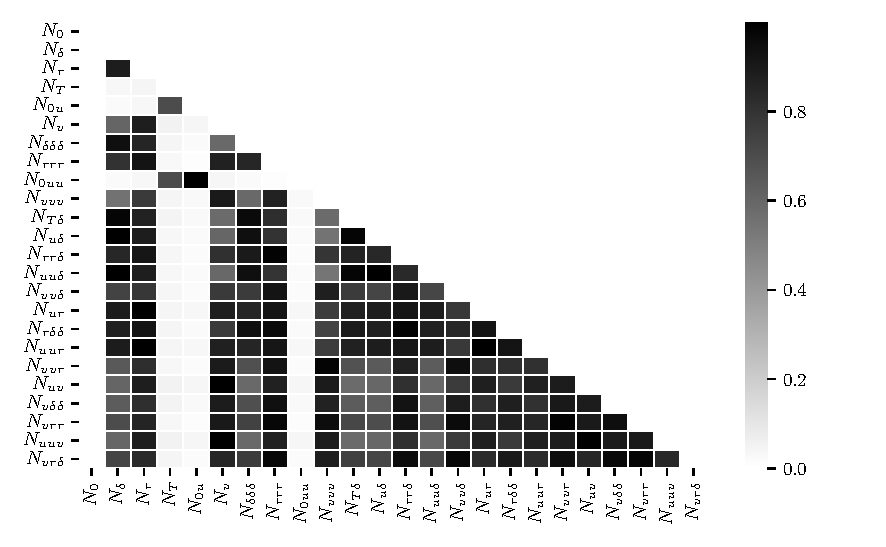
\includegraphics[width=1.0\textwidth]{kappa/images/10.pdf}
\caption{Absolute correlation between the features in the wPCC yaw moment regression of AVMM.}\label{fig:ncorr}
\end{figure}
Therefore, simulations of the validation cases were only possible using the MAVMM. 
The MAVMM model was retrained on the joined test and validation data set to obtain the final prediction model which was used to predict the turning circle test data set as shown in \autoref{fig:track-plot-testing-sim}. Advance and tactical diameter \cite{imoStandardsShipManoeuvrability2002} from the prediction differs by 4\% and 1\%. Monte Carlo simulations with alternative realizations of the regression, considering the uncertainty in the regressed parameters, are also displayed in these figures. The alternative realizations have similar simulation results to the model with mean values of the regression (black line).
\begin{figure}[ht]
\centering
\includegraphics[width=0.90\textwidth]{kappa/images/11.pdf}
\caption{Turning circle test case for wPCC, track plots from model test and simulation.}\label{fig:track-plot-testing-sim}
\end{figure}
\begin{figure}[ht!]
\centering
\includegraphics[width=0.90\textwidth]{kappa/images/12.pdf}
\caption{Turning circle test case for wPCC, time series from model test and simulation.}\label{\detokenize{06.10_results_wpcc:fig-testing-sim}}\end{figure}
\clearpage
A similar study was conducted for the KVLCC2 test case. \autoref{fig:kvlcc2_datasets}) shows how the datasets have been divided.
\begin{figure}[h!]
\centering
\includegraphics[width=1.0\textwidth]{kappa/images/4.pdf}
\caption{KVLCC2 training, validation and testing datasets.}\label{fig:kvlcc2_datasets}
\end{figure}

\noindent Results from the final prediction of the turning circle test are shown in  \hyperref[\detokenize{06.20_results_kvlcc2:fig-kvlcc2-track-plot-testing-sim}]{\autoref{\detokenize{06.20_results_kvlcc2:fig-kvlcc2-track-plot-testing-sim}}}, \hyperref[\detokenize{06.20_results_kvlcc2:fig-kvlcc2-testing-sim}]{\autoref{\detokenize{06.20_results_kvlcc2:fig-kvlcc2-testing-sim}}}. The prediction is conducted using simulation with the MAVMM trained on the training and validation datasets. Monte Carlo simulations with alternative realizations of the regression are also displayed in this figure. The alternative realizations are very similar to the model with mean values of the regression (black line).
\begin{figure}[h!]
\centering
\includegraphics[width=1.0\textwidth]{kappa/images/17.pdf}
\caption{Comparison between the predicted turning circle test with MAVMM trained on HSVA data and MARIN model test results for KVLCC2.}\label{\detokenize{06.20_results_kvlcc2:fig-kvlcc2-track-plot-testing-sim}}\end{figure}
\begin{figure}[h!]
\centering
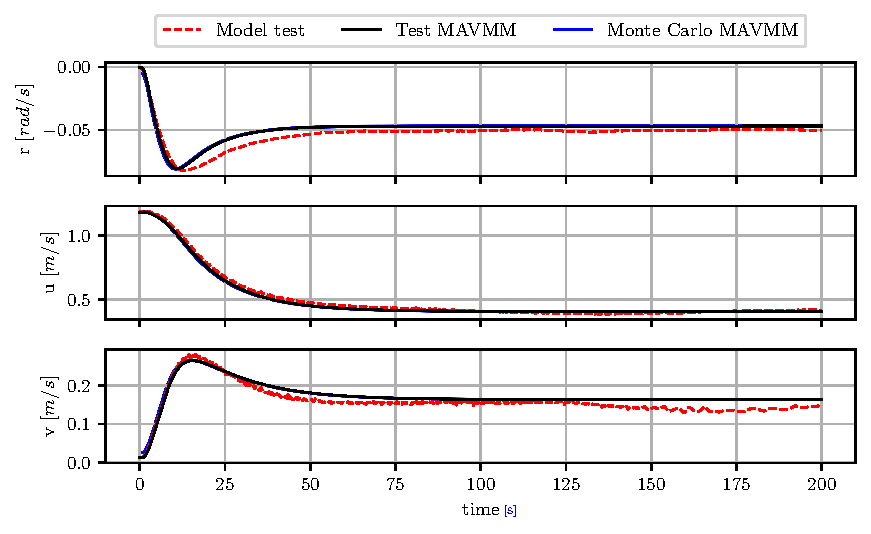
\includegraphics[width=1.0\textwidth]{kappa/images/18.pdf}
\caption{Comparison between the predicted turning circle test with MAVMM trained on HSVA data and MARIN model test results for KVLCC2.}\label{\detokenize{06.20_results_kvlcc2:fig-kvlcc2-testing-sim}}\end{figure}
The predicted advance and tactical diameters differ by 2\% and 5\%, which is considered acceptable because of the margin of the IMO standard limits (which are also displayed in this table). The results are also closer to the model tests than a similar study conducted for the KVLCC2 \cite{heNonparametricModelingShip2022}.
